В данном листке описаны результаты численной диагонализации 
гамильтониана 2D топологического изолятора для нескольких 
физических ситуаций.
\section{Огибание препятствия краевыми модами}
Как известно, краевые моды не могут рассеиваться назад на потенциальных примесях. 
В связи с этим интересно увидеть, что происходит, когда краевая мода <<натыкается>> на
потенциальное препятствие. Логично предположить, что она будет огибать это препятствие
независимо от его формы и глубины. Численная диагонализация это подтверждает.
\begin{figure}[h]
    \centering
    \begin{minipage}[h]{0.4\linewidth}
        \fbox{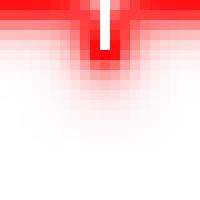
\includegraphics[width=1.\linewidth]{obstacle_1.png}}
    \end{minipage}
    \hfill
    \begin{minipage}[h]{0.4\linewidth}
        \fbox{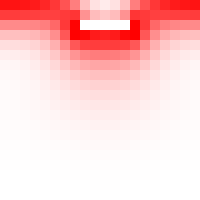
\includegraphics[width=1.\linewidth]{obstacle_2.png}}
    \end{minipage}
    \caption{
        Квадрат амплитуды волновой функции краевого состояния, огибающего препятствия. 
        Размер решётки --- $20\times20$, по горизонтальной оси наложены периодические
        граничные условия.
    }
\end{figure}
\section{Эффекты потенциального беспорядка}
Аналогично предыдущему, потенциальный беспорядок не должен разрушать краевые состояния.
Это верно даже для сильного беспорядка.
\begin{figure}[h]
    \centering
    \begin{minipage}[h]{0.4\linewidth}
        \fbox{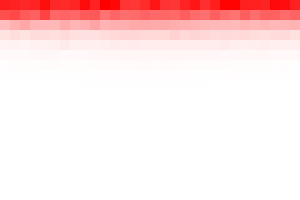
\includegraphics[width=1.\linewidth]{dis_edge_state_1.png}}
        \caption{
            Волновая функция краевого состояния с беспорядком.
            Параметры модели: $\xi, m, t = -0.2, 1, 0.4$, сила беспорядка --- $0.5$.
            }
    \end{minipage}
    \hfill
    \begin{minipage}[h]{0.4\linewidth}
        \fbox{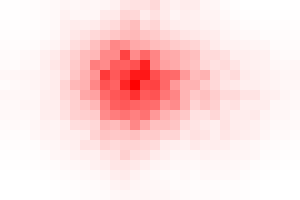
\includegraphics[width=1.\linewidth]{dis_bulk_state.png}}
        \caption{
            Волновая функция объемного состояния с беспорядком для тех же параметров.
            }
    \end{minipage}
\end{figure}
 \section{Граница области с беспорядком и <<чистой>> области}
 Ещё не очень понятно, как это будет работать. 
\section{Локализация магнитным беспорядком}
Магнитный беспорядок, как нарушающий $T$--симметрию, приводит к рассеянию состояний
с двумя компонентами спина друг в друга. Это приводит к локализации краевых состояний,
что продемонстрировано на рисунках.
\begin{figure}[h]
    \centering
    \begin{minipage}[h]{0.9\linewidth}
        \fbox{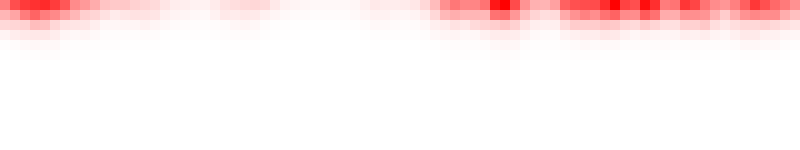
\includegraphics[width=1.\linewidth]{mgn_edge_st_1.png}}
    \end{minipage}
    \begin{minipage}[h]{0.9\linewidth}
        \fbox{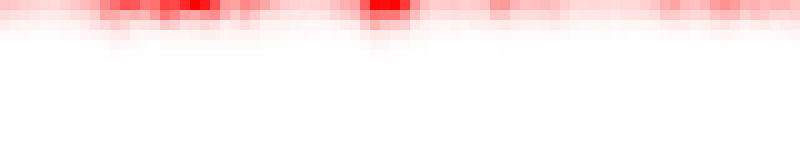
\includegraphics[width=1.\linewidth]{mgn_edge_st_2.png}}
    \end{minipage}
    \begin{minipage}[h]{0.9\linewidth}
        \fbox{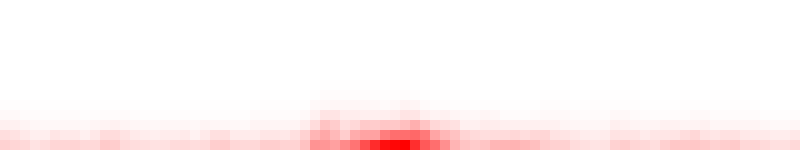
\includegraphics[width=1.\linewidth]{mgn_edge_st_3.png}}
    \end{minipage}
    \caption{
        Волновые функции краевых состояний с магнитным беспорядком 
        для тех же параметров.
        }
\end{figure}
